\documentclass{article}
\usepackage[utf8]{inputenc}

\title{BDSA00}
\author{Freja Bruun Vanggaard}
\date{September 2021}
\usepackage{graphicx}

\begin{document}
\maketitle

\section{Algorithm description and illustration}

\begin{figure}[h!]
\centering
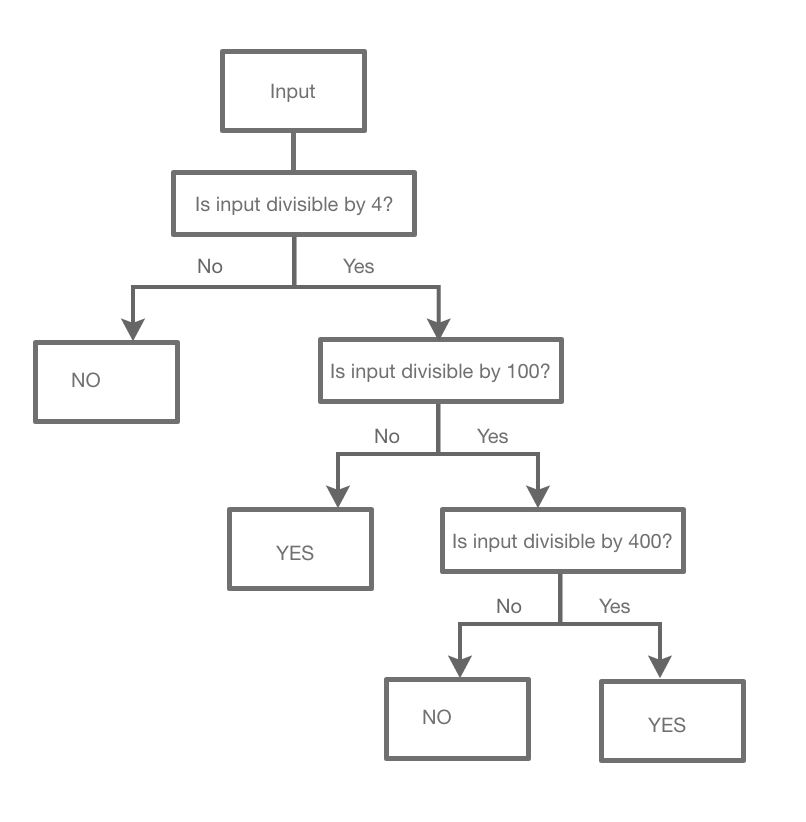
\includegraphics[scale=0.325]{UML1.png}
\caption{YES and NO in the boxes refers to the answer to: Is the input a leap year?}
\end{figure}


So first the given year is checked to see if it is divisible by 4. If it is not divisible by 4 there is no way it can be a leap year as seen in the diagram following the arrow stating no. In case it is divisible by 4, we have to check if it is divisible by 100, because this might invalidate the leap year state. If it is not divisible by 100, it is safe to assume that it is a leap year. But if it is also divisible by 100, then we have to check if it divisible by 400, this check is the last possible one in the diagram. If it is also divisible by 400, then it is a leap year. If it is not divisible by 400, we can see that the previous check (divisible by 100) validated to yes, and the result therefore ends ud not being a leap year.

All of this is seen on the (attempted) UML diagram, illustrated by the arrows showing the paths that are taken in case of the different truth value evaluations. 

\end{document}
